\documentclass[aspectratio=169]{beamer}


\usetheme{default}
\setbeamertemplate{navigation symbols}{}
\setbeamertemplate{enumerate item}{\color{navy}\arabic{enumi}.}
\setbeamertemplate{itemize item}{\color{black}\textbullet}
\setbeamertemplate{itemize subitem}{\color{black}\textbullet}
\usepackage{booktabs}
\usepackage{xcolor}
\usepackage{tikz}
\usetikzlibrary{shapes,arrows,positioning}
\definecolor{navy}{RGB}{0, 0, 128}
\definecolor{lightblue}{RGB}{230,240,250}
\definecolor{darkgreen}{RGB}{0,100,0}
\definecolor{lightgreen}{RGB}{230,250,230}
\newcommand{\highlight}[1]{\colorbox{lightblue}{$\displaystyle\textcolor{navy}{#1}$}}
\newcommand{\highlighttext}[1]{\colorbox{lightblue}{\textcolor{navy}{#1}}}
\newcommand{\highlightgreen}[1]{\colorbox{lightgreen}{$\displaystyle\textcolor{darkgreen}{#1}$}}

\begin{document}

\begin{frame}

CCPs work because we observe choices in data

\bigskip

\onslide<2->{
For observed state $(x,s)$, estimate probability of action $j$:

$$
p_{jt}(x,s) = \frac{\sum_i d_{ijt}1[X_{it}=x, S_{it}=s]}{\sum_i 1[X_{it}=x, S_{it}=s]}
$$
}

\bigskip


\onslide<3->{
Use these probabilities to construct expected future values

\bigskip

Leverage finite dependence, renewal, or terminality to avoid solving value functions
}

\onslide<3->{
\bigskip

$p_{jt}$'s inform us about the future value of taking certain actions at certain states
}

\end{frame}





\begin{frame}

\textcolor{navy}{Problem:} What if key states are unobserved?

\bigskip

\onslide<2->{
Cannot compute $p_{jt}(x,s)$ when $s$ unobserved
}

\onslide<3->{
$$
p_{jt}(x,\highlight{s}) = \frac{\sum_i d_{ijt}1[X_{it}=x, \highlight{S_{it}=s}]}{\sum_i 1[X_{it}=x, \highlight{S_{it}=s}]}
$$
}

\bigskip

\onslide<4->{
This arises routinely in DDC models:
\bigskip\par
}
\begin{itemize}
\itemsep1.5em
\item<5-> Dynamic selection
\item<6-> Serially correlated unobservables
\end{itemize}
\end{frame}


\begin{frame}
\centering
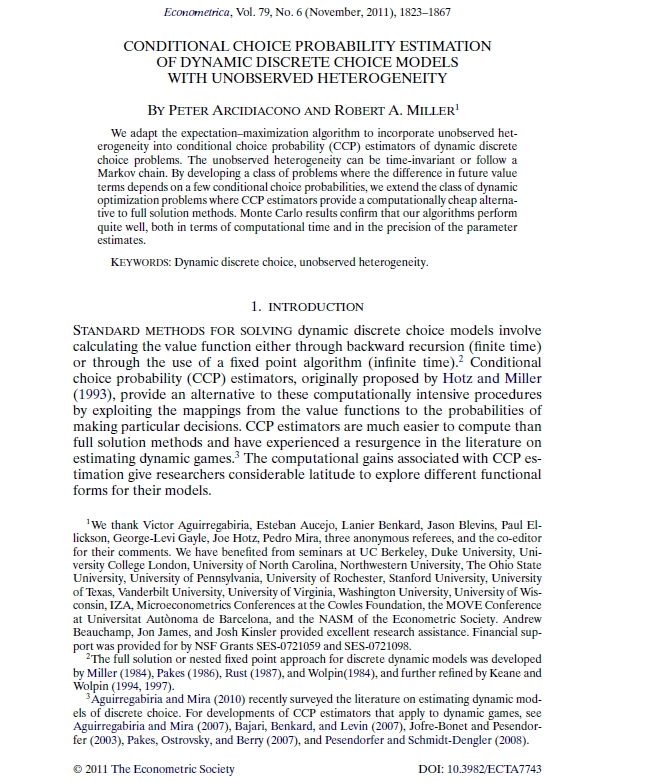
\includegraphics[width=0.5\textwidth]{ArcidiMiller_cover.jpg}
\end{frame}



\begin{frame}

\textcolor{navy}{Solution:} Assume $S$ is finite and use EM algorithm

\bigskip

Assume $R$ unobserved types with probabilities $\pi_s$

\bigskip

\onslide<2->{
Key insight: Use posterior probability $q_{is}$ as weight

$$
q_{is} = \frac{\pi_s\prod_{t=1}^T\mathcal{L}_{ist}(\theta_s)}{\sum_{s'=1}^R\pi_{s'}\prod_{t=1}^T\mathcal{L}_{is't}(\theta_{s'})}
$$

\bigskip

$q_{is}$ = probability individual $i$ is type $s$ given observed choices
}

\end{frame}

\begin{frame}

Weighted CCP estimator replaces indicator with posterior type probability:

\bigskip

$$
p_{jt}(x,s) = \frac{\sum_i d_{ijt}\highlight{q_{is}}1[X_{it}=x]}{\sum_i \highlight{q_{is}}1[X_{it}=x]}
$$

\bigskip

\onslide<2->{
Now treats unobserved type as observed (with weights)

\bigskip

Can estimate CCPs conditional on unobserved states
}

\end{frame}

\begin{frame}

EM Algorithm for CCP estimation at iteration $m$:

\bigskip

\textcolor{navy}{E-step:} Given $\theta^m$, $\pi^m$, $p^m$, compute

$$
q_{is}^{m+1} = \frac{\pi_s^m\prod_{t=1}^T\mathcal{L}_{ist}(\theta^m, p^m)}{\sum_{s'=1}^R\pi_{s'}^m\prod_{t=1}^T\mathcal{L}_{is't}(\theta^m, p^m)}
$$

\bigskip

\onslide<2->{
\textcolor{navy}{M-step:} Given $q^{m+1}$, update

$$
p_{jt}^{m+1}(x,s) = \frac{\sum_i d_{ijt}q_{is}^{m+1}1[X_{it}=x]}{\sum_i q_{is}^{m+1}1[X_{it}=x]}
$$

$$
\theta^{m+1} = \arg\max_\theta \sum_i\sum_s\sum_t q_{is}^{m+1}\log\mathcal{L}_{ist}(\theta, p^{m+1})
$$
}

\end{frame}

\begin{frame}

Key benefits of EM + CCP approach:

\bigskip

\begin{itemize}
\itemsep1.5em
\item<2-> No backward recursion needed (leverage finite dependence/renewal/terminality)
\item<3-> Maximization step treats types as observed
\item<4-> Maintains additive separability for sequential estimation
\item<5-> Computational tractability despite unobserved heterogeneity
\end{itemize}

\end{frame}

\begin{frame}

Alternative CCP update: Use structural model

\bigskip

Instead of weighted empirical frequencies, use likelihood:

$$
p_{jt}^{m+1}(x,s) = \ell_j(x, s; \theta^m, \pi^m, p^m)
$$

\bigskip

\onslide<2->{
Where $\ell_j$ comes from choice probabilities implied by model

\bigskip

For example, with T1EV errors:

$$
p_{jt}(x,s) = \frac{\exp(v_j(x,s))}{\sum_k \exp(v_k(x,s))}
$$

\bigskip

Both methods converge to same estimates
}

\end{frame}


\end{document}